\chapter{理论基础及相关技术概述}



\section{Linux 内存管理技术}

\subsection{物理内存管理}


\begin{figure}[h]
    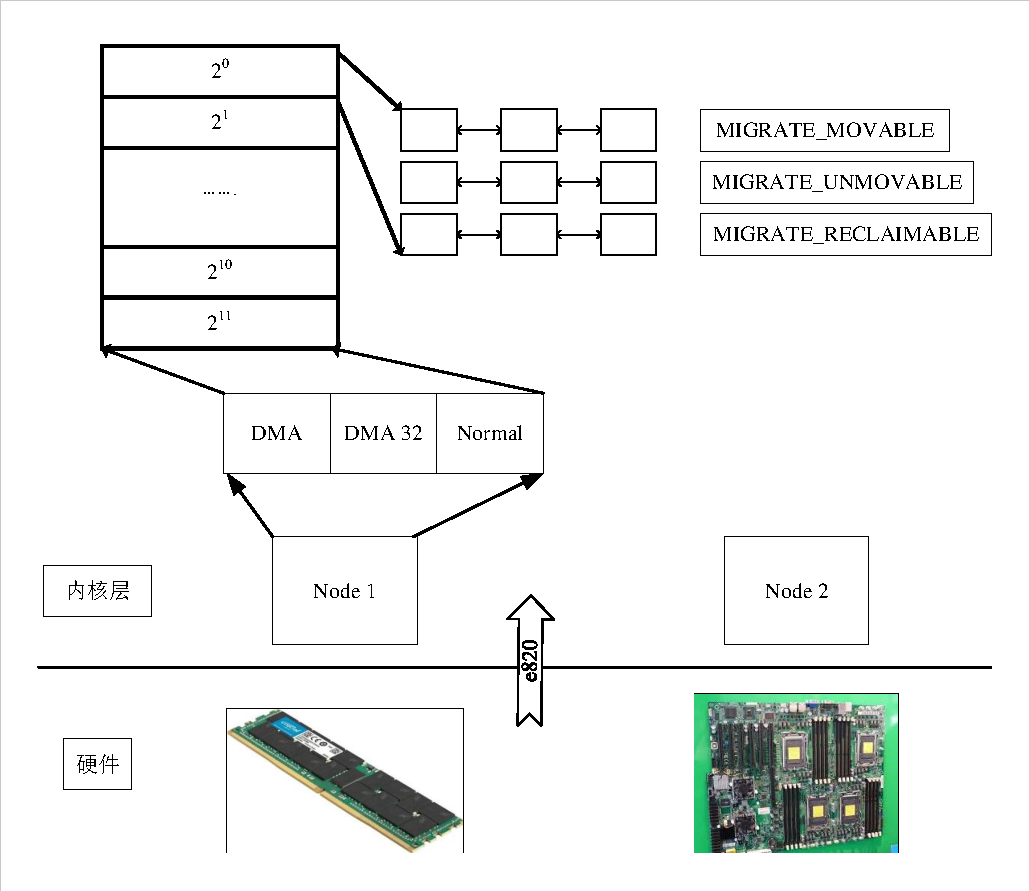
\includegraphics{物理内存管理.pdf}
    \caption{物理内存管理}
    \label{物理内存管理}
\end{figure}



如上图\ref{物理内存管理}所示,在最底层的硬件基础上,系统首先需要准确掌握物理内存的具体信息。如图所示,这一过程通过BIOS的e820协议实现。该协议作为硬件和操作系统之间的桥梁,提供了系统物理内存的详细信息,包括内存大小、物理地址范围以及内存区域的可用性状态。这些基础信息构成了整个内存管理体系的基石,为上层管理机制提供了必要的硬件抽象。

在硬件架构层面,图中展示了典型的非一致内存访问(Non-Uniform Memory Access,NUMA)架构,包含Node 1和Node 2两个独立节点。每个节点都配备了独立的处理器和本地内存资源,这种设计充分考虑了内存访问的局部性原理。由于访问本地内存的延迟显著低于远程访问,系统会优先利用本地节点的内存资源,从而有效提升整体性能。这种架构设计在现代服务器系统中得到了广泛应用,为大规模并行计算提供了强有力的硬件支持。

基于对物理内存的准确认知,Linux实现了精细的内存区域管理机制。如图所示,系统将物理内存空间划分为DMA区域、DMA32区域和Normal区域。这种分区设计源于硬件发展的历史特征:DMA区域(16MB以下)主要用于兼容早期的ISA设备,DMA32区域(4GB以下)则满足32位设备的寻址需求,而Normal区域则为现代64位设备提供更大的地址空间。这种分层设计不仅确保了系统对各类硬件设备的良好兼容性,还提供了高效的内存分配机制。

在内存管理的核心层面,Linux实现了多级页面大小的精细化控制。如图中所示,系统支持从$2^0$到$2^{11}$不等的页面大小,这种灵活的设计适应了不同场景的需求。小页面配置适用于精细化的内存管理,能够有效减少内存碎片,提高空间利用率;而大页面配置则主要用于需要大块连续内存的场景,通过减少页表项数量和提升TLB命中率来优化系统性能。这种多级页面设计体现了Linux内存管理的灵活性和高效性。

在这一体系的最上层,Linux创新性地引入了内存迁移类型系统。如图右上角所示,该系统将内存页面分为MIGRATE\_MOVABLE(可移动页面)、MIGRATE\_UNMOVABLE(不可移动页面)和MIGRATE\_RECLAIMABLE(可回收页面)三类。可移动页面主要分配给用户空间应用,支持物理地址的动态调整;不可移动页面用于存储包含物理地址引用的内核数据结构;而可回收页面则包含可被系统回收的内容,如页面缓存等。这种分类机制直接服务于内存碎片管理,提供了灵活的内存资源调配能力。

通过这种层次化的设计,Linux内存管理系统实现了从硬件到软件的无缝衔接。

\subsection{资源限制 CGroup}






资源管理是操作系统的核心功能之一,而 cgroup v2 作为 Linux 内核的新一代资源管理机制,通过统一的层级结构提供了精细化的资源控制能力。在内存管理领域,cgroup v2 依托其内存控制器实现了全方位的资源限制与追踪。该控制器不仅可以监控用户空间内存、内核数据结构、TCP 套接字缓冲区等多种内存使用情况,还能通过挂载选项 memory\_hugetlb\_accounting 来支持对 HugeTLB 内存的管理。

内存限制的实现采用了分层控制策略,通过不同级别的限制机制来保障系统稳定性。硬限制通过写入 memory.max 接口来设置,例如设置 1GB 的限制可通过命令 `echo 1073741824 > memory.max` 实现。当进程组内存使用达到此上限时,系统将触发 OOM Killer 进行资源回收。软限制则通过 memory.high 接口设置,如 `echo 805306368 > memory.high` 设置 750MB 的预警阈值。当内存使用超过此值时,系统会增加内存回收的频率和力度,但不会直接终止进程,为管理员预留了干预空间。同时,系统引入了 memory.min 和 memory.low 作为保护机制,分别通过 `echo 104857600 > memory.min` 和 `echo 209715200 > memory.low` 设置 100MB 的硬保护和 200MB 的软保护限制,确保关键业务的内存需求。

在资源组织架构上,cgroup v2 实现了严格的层级管理模型。每个进程仅能归属于一个 cgroup,资源分配严格遵循自顶向下的原则。子 cgroup 获得的资源受限于父 cgroup 的分配,这种层级关系通过目录结构直观体现。特别值得注意的是,内存区域的归属关系与进程的迁移状态相互独立,即便进程被迁移到新的 cgroup,其已分配的内存仍计入原 cgroup,这一特性保证了资源追踪的准确性。

当系统需要主动进行内存回收时,可以通过 memory.reclaim 接口触发。具体操作为向该接口写入待回收的字节数,如 `echo 52428800 > memory.reclaim` 来回收 50MB 内存。回收过程支持异步操作,系统会优先回收不活跃的缓存页和匿名页,同时考虑 memory.low 设定的保护值。若要在发生 OOM 时对整个 cgroup 进行管理,可通过设置 `echo 1 > memory.oom.group` 来启用组级别的 OOM 控制。

在容器化环境中,cgroup v2 的内存管理机制发挥着核心作用。容器运行时通过配置 cgroup 参数来实现资源隔离,例如在 Docker 中可使用 `--memory` 和 `--memory-reservation` 参数分别对应 memory.max 和 memory.high 的设置。管理员能够通过 memory.current 和 memory.stat 接口实时监控资源使用状况,其中 memory.current 提供当前内存使用量,而 memory.stat 则提供包括活跃页面数、缓存大小等详细统计信息。这些数据对于系统调优和故障诊断具有重要参考价值。

为提升资源管理的精确性,cgroup v2 还引入了一系列高级特性。memory.oom.group 的引入使得 OOM 处理更具可控性,而 memory.reclaim 则为系统提供了主动干预的能力。此外,memory.numa\_stat 接口的引入也使得在 NUMA 架构下的内存管理更为高效。这些特性的有机结合,构建了一个完整的内存资源管理体系,为现代云原生应用提供了可靠的运行基础。

\subsection{直接页面回收机制}
\label{sec:直接页面回收机制}

Linux中使用伙伴系统来管理物理内存,用户态程序申请的虚拟内存在第一次的使用的时候会缺页中断然后有申请物理的物理页面,然后建立页表映射。

当系统内存使用量达到预设阈值,例如 Linux 内核配置的内存水位线(watermark)或 cgroup 设定的内存限制时,将触发内存页回收机制。\_\_alloc\_pages\-\_direct\_reclaim
函数是执行直接内存回收的核心函数,其主要职责是从节点(node)、内存域(zone)以及最近最少使用(LRU)链表中回收内存页,以缓解内存压力。

在 try\_to\_free\_pages 函数中,系统首先设定内存回收的优先级,并初始化扫描控制结构体 scan\_control。scan\_control 结构体用于指导内存回收过程,其中包含了回收的优先级、目标等参数。随后,系统根据 scan\_control 结构体以及其他相关参数,确定需要扫描的zone、节点node以及 cgroup。

接下来,流程进入 get\_scan\_count 函数。该函数的核心功能是计算文件页和匿名页的回收比例,并根据系统负载和内存压力情况,决定本次回收操作主要针对文件页还是匿名页,以及各类页面的回收数量。这种策略性的回收比例调整,旨在平衡系统性能和内存回收效率。

最终,内存回收操作在 shrink\_list 函数中执行。该函数针对选定的 LRU 链表进行内存页回收。针对活动页链表,shrink\_list 函数首先隔离部分页面到一个临时链表。随后,通过调用 page\_referenced() 函数检查被隔离页面的访问位(accessed bit)。若页面在近期被访问过,则表明其仍然活跃,page\_referenced() 函数会设置页面的访问位,并将该页面降级到非活动页链表,延迟其回收。对于未被访问的页面,则可能直接进行回收。

对于非活动页链表,shrink\_list 函数同样会隔离可回收的页面。这些页面是被认为是相对不活跃的内存页,是内存回收的主要目标。 shrink\_list 函数会对隔离的非活动页进行进一步的检查和回收操作,例如将文件页写回磁盘,释放匿名页并可能将其交换到交换空间等,最终释放内存页,缓解系统内存压力。

\subsection{冷热页识别机制}

\section{本章小结}